\documentclass[11pt]{article}

\usepackage{times}
\usepackage{alltt}
\usepackage{graphicx}
\usepackage{url}

\bibliographystyle{plain}

%% Page layout
\oddsidemargin 0pt
\evensidemargin 0pt
\textheight 600pt
\textwidth 469pt
\setlength{\parindent}{0em}
\setlength{\parskip}{1ex}

%% ccode environment- for displaying formatted C code (c2tex) 
\newenvironment{ccode}%
{\small}%
{}

%% tty - for displaying TTY input and output
\newenvironment{tty}%
{\small\begin{alltt}}%
{\end{alltt}}


\begin{document}
\title{CS33, Spring 2020\\
Parallel Lab - Intro to Multi-threading\\
}

\author{}%Spring 2020: Attiano Purpura-Pontoniere
\date{Due: Friday, June 5th at 11:59pm. }

\maketitle

\section{Getting Started}
The goal of this lab is to accelerate some poorly written code we have provided. You should consider using the optimization techniques (both single threaded and multithreaded) we have covered in class to accelerate this code.
\begin{enumerate}
    \item To start, grab the lab folder - this command will copy the lab directory to your current working directory:
        \begin{tty}
        cp -r /w/class.1/cs/cs33/csbin/ParallelLab .
        \end{tty}
    \item To compile the code:\\
            \textbf{make all}: This will create the Test executable.\\
            \\
          Before re-compiling:\\
            \textbf{make clean}: This will delete all object files.\\
    \item Once you have successfully compiled, you can run the executable with:
        \begin{tty}
            ./Test
        \end{tty}
    \item Each time you modify parallel.c, you need to recompile the program using the steps detailed in 2. above. 
    \item Remember to add your name, UCLA ID and email details in the comment section in the parallel.c file.
    \item You are allowed to modify parallel.c for this lab. You \textbf{should not edit any other files except parallel.c} as we are going to measure your parallel version against our sequential version (we may change the initial state of the input matrix so do not optimize for the specific data or functions in main.c). We will also leave utils.h and the makefile unchanged.
    \item We will use \textbf{lnxsrv04.seas.ucla.edu} to evaluate your code. This machine is an 8-core system with hyperthreading (e.g. 16 virtual cores). You may develop your code elsewhere, but we will only grade based on the performance you obtain on lnxsrv04.seas.ucla.edu. The performance of your optimized code will depend on the load (what else is running) on the system. You can use programs like \textbf{top} to see the load of the system. After top starts press 1 to see the load on each core of the machine. We will run on an uncontested machine when we evaluate your code to ensure it is not impeded by other programs.
    \item SEASnet servers are shared by all students in the engineering departments, including your fellow CS 33 students. When multiple students are running their programs the performance of your program may be drastically lower. To avoid testing problems due to high machine contention, START EARLY!



\end{enumerate}

\section{Submission}
\begin{enumerate}
    \item Submit \textbf{only parallel.c} via CCLE.
    \item Remember to \textbf{add your name, UCLA ID, and email in the comment section in parallel.c}
    \item The deadline for submission is \textbf{Friday, June 5th, 2020 11:59pm.}
\end{enumerate}


\section{Grading}
Grading will be done on lnxsrv04.seas.ucla.edu to prevent any other processes from interfering with the timing results. You will receive points proportional to the speed up. You receive 28.75 points for the first .5x speedup, then 14.25 points for each .5x speedup after that until 3.5x. Any speedup greater than 3.5x speed-up will result in extra credit. The extra credit will be awarded as half-points for any integer speed-up over 3.5x:
\begin{itemize}
    \item \textbf{$>$3.5x} speed up: 100/100 points
    \item \textbf{3 - 3.49x} speed up: 85.75/100 points
    \item \textbf{2.5 - 2.99x} speed up: 71.5/100 points
    \item \textbf{2 - 2.49x} speed up: 57.25/100 points
    \item \textbf{1.5 - 1.99x} speed up: 43/100 points
    \item \textbf{1 - 1.49x} speed up: 28.75/100 points
    \item $<1x$ speed up: 0/100
    \item The max extra credit for this lab is 15\% for a speed up $>3.5$. Extra credit will calculated with the following exponential decay equation: $ 15*(1-2*e^{-\frac{floor(your\_speedup - 3.5)}{2.0}})$\\
    
    \item Correctness is based off the behavior of $work\_it\_par()$ matching $work\_it\_seq()$. This is determined by comparing the values printed by both functions, the values returned by both functions, and the data manipulated by both functions, e.g. the output arrays match. Float values like those printed by the Monte Carlo pi loop are acceptable within a tolerance of $\pm.005$
    
\end{itemize}
\section{Notes}
\begin{itemize}
    \item Higher DIM values will result in longer run-time but more speedup. We will test at DIM = 500, if you run the given poorly optimized code with DIM = 500 it will take approximately 1.5 minutes to run ./Test on an empty server, and considerably longer on a crowded server. Also increasing DIM will result in a segfault as you are asking to malloc too much space on the heap.
    \item \textbf{DO NOT ATTEMPT TO CIRCUMVENT OPTIMIZATION BY RETURNING THE RIGHT VALUE DIRECTLY, WE WILL TEST FOR THIS, AND SCORE YOU 0.}
    \item \textbf{PLEASE DO NOT LET YOUR CODE ENTER AN INFINITE LOOP, THIS WILL STALL THE AUTOGRADER AND MAKE ME MANUALLY HAVE TO SCORE YOU 0.}
    \item I was able to get it to compile on lnxsrv03.seas.ucla.edu and lnxsrv04.seas.ucla.edu I had errors about "multiple definitions" when I tried compiling on lnxsrv06.seas.ucla.edu and lnxsrv10.seas.ucla.edu
    \item \textbf{YOU WILL RECEIVE A SCORE OF 0 IF:}
        \begin{enumerate}
            \item Your code doesn't compile on lnxsrv04.seas.ucla.edu or lnxsrv03.seas.ucla.edu
            \item Your code does not return/output the expected values
            \item Your code enters an infinite loop
            \item Your code segfaults or otherwise produces unexpected behavior
        \end{enumerate}
        
    \item Correct output looks like:
    \begin{figure}[h]
    \centering
        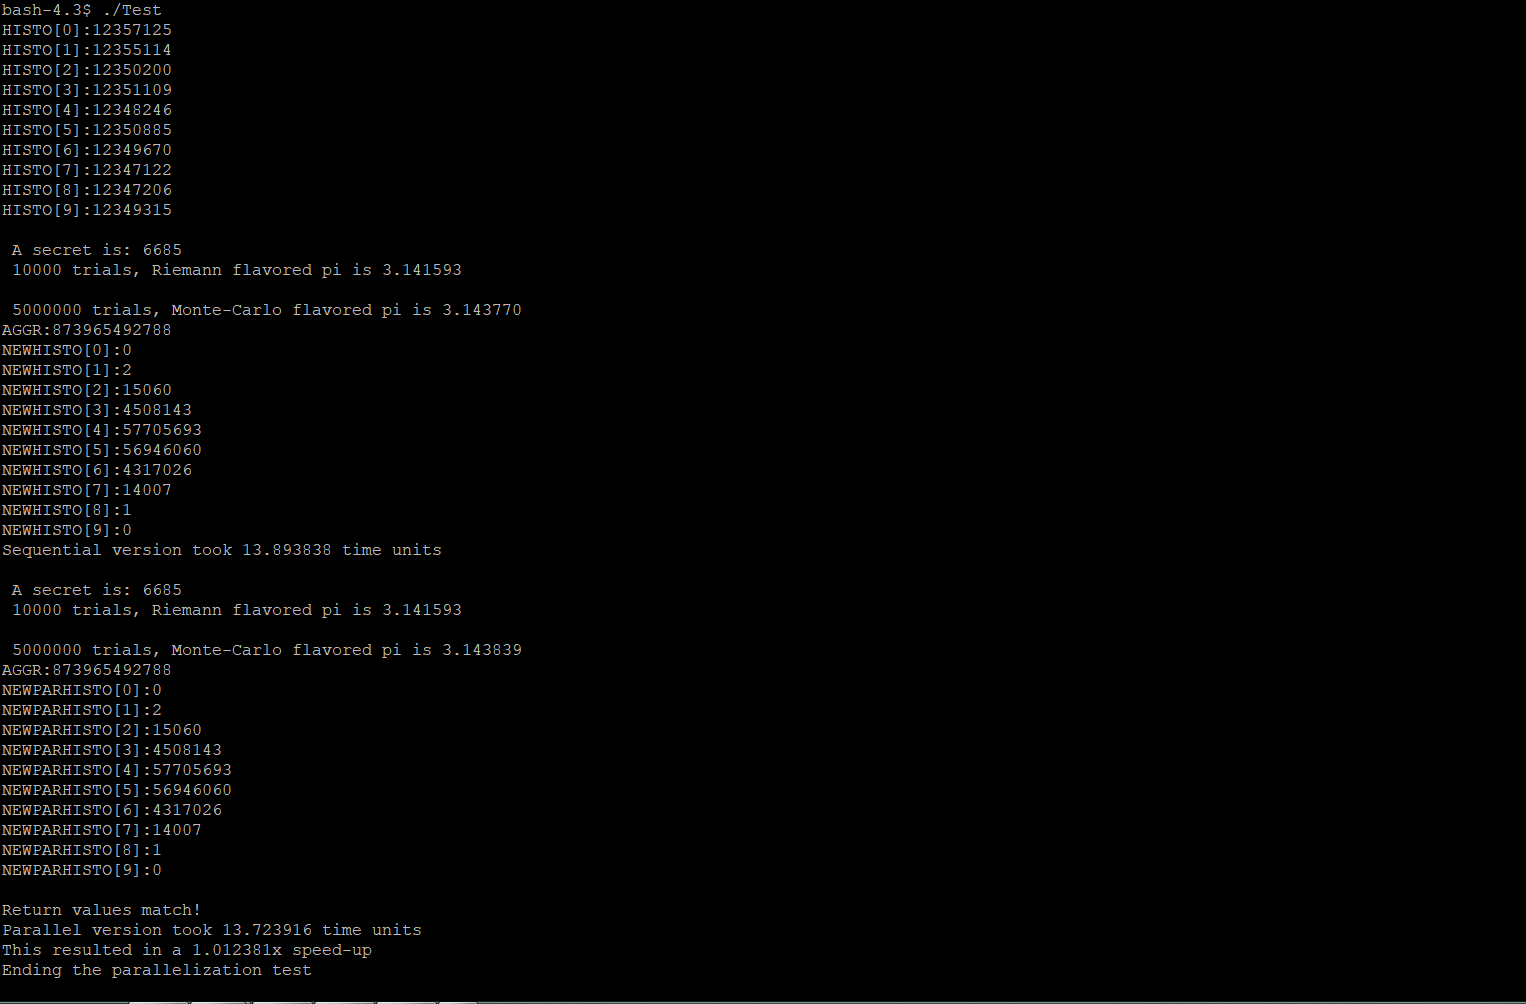
\includegraphics[width=0.75\textwidth]{correct_output.PNG}
        \caption{./Test Correct output reflecting correct behavior}
        \label{fig:test1}
    \end{figure}
\end{itemize}

\vspace{180pt}
\section{Hints}
\begin{itemize}
    \item You can use the optimization techniques we have covered in class, including loop tiling, OpenMP, code motion, etc.
    \item It is best to test on a server without other people testing as that will affect your speedup. For example, if there is a high load during the sequential runtime of your code and a low load during the parallel runtime it will make you think you have achieved a higher speed up as your parallel code will run faster because of a smaller load. Find a server that works for you without anyone and then once you have your final results, test on lnxsrv04.seas.ucla.edu to confirm.
\end{itemize}



\end{document}
